\documentclass[a4paper,UKenglish]{lipics-v2016}
 
\usepackage{microtype}

\bibliographystyle{plainurl}

\newcommand{\R}{\mathbb{R}}
\newcommand{\C}{\mathbb{C}}
\newcommand{\CP}{\hat{\mathbb{C}}}

\title{Exploring Circle Packing Algorithms\footnote{This work was partially supported by the National Science Foundation under grants CCF-1525978 and CCF-1464379.}}
\titlerunning{Exploring Circle Packing Algorithms}
 
\author[1]{Kevin Pratt}
\author[2]{Connor Riley}
\author[3]{Donald R.~Sheehy}
\affil[1]{University of Connecticut\\
  \texttt{kevin.pratt@uconn.edu}}
\affil[2]{University of Connecticut\\
  \texttt{connor.riley@uconn.edu}}
\affil[3]{University of Connecticut\\
  \texttt{don.r.sheehy@gmail.com}}

\authorrunning{K.\,Pratt, C.\,Riley, and D.\,R.\,Sheehy}

\Copyright{Kevin Pratt, Connor Riley, Donald R.~Sheehy}

\subjclass{F.2.2 Nonnumerical Algorithms and Problems---Geometrical problems and computations.}

\keywords{Computational Geometry, Processing, Javascript, Visualization, Incremental Algorithms}

\EventEditors{ Fekete and Anna Lubiw}
\EventNoEds{2}
\EventLongTitle{32nd International Symposium on Computational Geometry (SoCG 2016)}
\EventShortTitle{SoCG 2016}
\EventAcronym{SoCG}
\EventYear{2016}
\EventDate{June 14-18, 2016}
\EventLocation{Boston, USA}
\EventLogo{}
\SeriesVolume{51}
\ArticleNo{69}  

\begin{document}

\maketitle

\begin{abstract}
  We present an interactive tool for visualizing and experimenting with different circle packing algorithms. 
  The source code can be found at: https://github.com/interl0per/CirclePacking
\end{abstract}

\section{Introduction}
\label{sec:introduction}

  The Koebe Embedding Theorem provides a wonderful link between questions of geometry, topology, combinatorics, and complex analysis.
  It states that every planar graph can be realized as the intersection graph of a collection of interior disjoint circles in the plane.
  That is, the vertices correspond to circles and two circles are tangent if and only if their corresponding vertices share an edge.
  Such a graph representation is called a circle packing.
  They have found application in computational geometry such as in a proof of the planar separator theorem~\cite{miller97separators} or for bounding eigenvectors of graph Laplacians~\cite{kelner06spectral}.
  
  Technically, circle packings exist for any planar graph, but it is often simpler algorithmically to work with $3$-connected, triangulated planar graphs and we will assume such graph throughout.
  There are several known algorithms for computing a circle packing from a given planar graph.
  Early proofs of the existence of circle packings were non-constructive, but the work of Colin de Verdiere\cite{colindeverdiere91principe} and others~\cite{mohar93polynomial,bobenko03variational} showed that circle packings can be computed by convex optimization, ushering in several different iterative algorithms.
  A good introduction to the mathematical and algorithmic aspects of circle packings can be found in the book by Stephenson~\cite{stephenson05introduction}.
  
  As shown in the work of Bobenko and Springborn, there are several different energy functionals that one could minimize to arrive at a circle packing~\cite{bobenko03variational}.
  However, there are simple heuristics that are not known to give correct algorithms, yet still seem to produce good circle packings. 
  We present a tool designed to make it easy to mix and match circle packing heuristics. 
  One can quickly generate a triangulated planar graph and then apply different heuristics to move it towards a circle packing representation.

\section{Background}
\label{sec:background}

  \textbf{Weighted Delaunay Triangulation.}
  Circle packings are closely related to several other well-known topics in computational geometry.
  The most notable, being \emph{weighted Delaunay triangulations}.  
  This is the dual to the so-called power diagram, a Voronoi diagram on the points where the (squared) distance to a circle $c$ with center $p$ and radius $r$ is defined to be $\pi_c(x)^2 := \|x-p\|^2 - r^2$.
  A circle packing representation of a graph realizes the graph as the weighted Delaunay triangulation where the vertices are the centers of the disks and the weights are the radii.
  
  \textbf{Equilibrium Stresses.}
    A \emph{stress} is an assignment of real numbers to edges that may be interpreted as spring constants.
    By Hook's Law, the magnitude of the force exerted by a spring is the spring constant times its length.
    A stress is an \emph{equilibrium stress} if for each vertex, the sum of the forces exerted on it by all its incident edges is exactly zero.
    
    Weighted Delaunay triangulations have another interpretation as projections of convex polyhedra in $\R^3$.
    The Maxwell-Cremona Correspondence implies that projections of convex polyhedra always admit an equilibrium stress that is nonnegative on all edges except those of the convex hull.
    Thus, an alternative (dual) perspective on circle packings is that rather than looking for the correct radii, one could look for the correct equilibrium stress.
    Given a stress, one finds the embedding by Tutte's algorithm.
    This involves solving one system of linear equations derived from the graph.
  
  \textbf{Stereographic Mappings and M\"{o}bius Tranformations.} 
    Weighted Delaunay triangulations can also be realized as stereographic projections of convex polyhedra.
    In the case of circle packings this polyhedron is sometime called the Koebe polyhedron.
    It has the interesting property that the edges are all tangent to a sphere.

  \begin{figure}[ht]
    \centering
      \includegraphics[width = 0.45\textwidth]{figures/3D.png}
      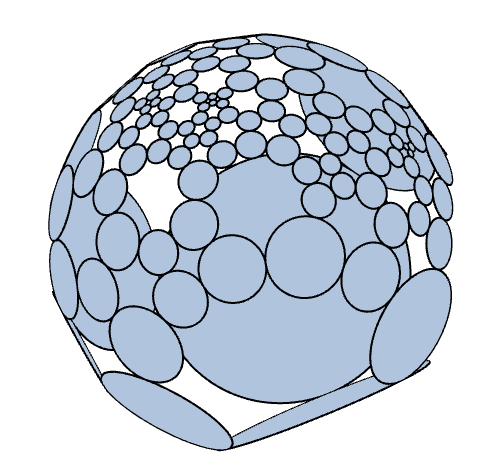
\includegraphics[width = 0.45\textwidth]{figures/3D_2.png}
    \caption{Stereographic projection of a circle packing.}
    \label{fig:3D}
  \end{figure}

  A \textbf{M\"{o}bius Transformation} of a plane can be obtained by performing the stereographic projection of the plane onto a sphere, then rotating or moving the sphere and then performing the stereographic projection back onto the plane. 
  Formally, a M\"{o}bius Transformation is a rational function defined on the extended complex plane $\CP = \C\cup\{\infty\}$ of the form:
  \begin{equation} 
  	f(z) = \frac{az+b}{cz+d}
  \end{equation}
  where $z\in\CP$ is a complex variable and $a,b,c,d\in\CP$ are complex numbers such that $ad - bc$ $\neq$ $0$.
  Circle packings in the plane are unique up to M\"{o}bius Transformation.
    \begin{figure}[ht]
      \centering
        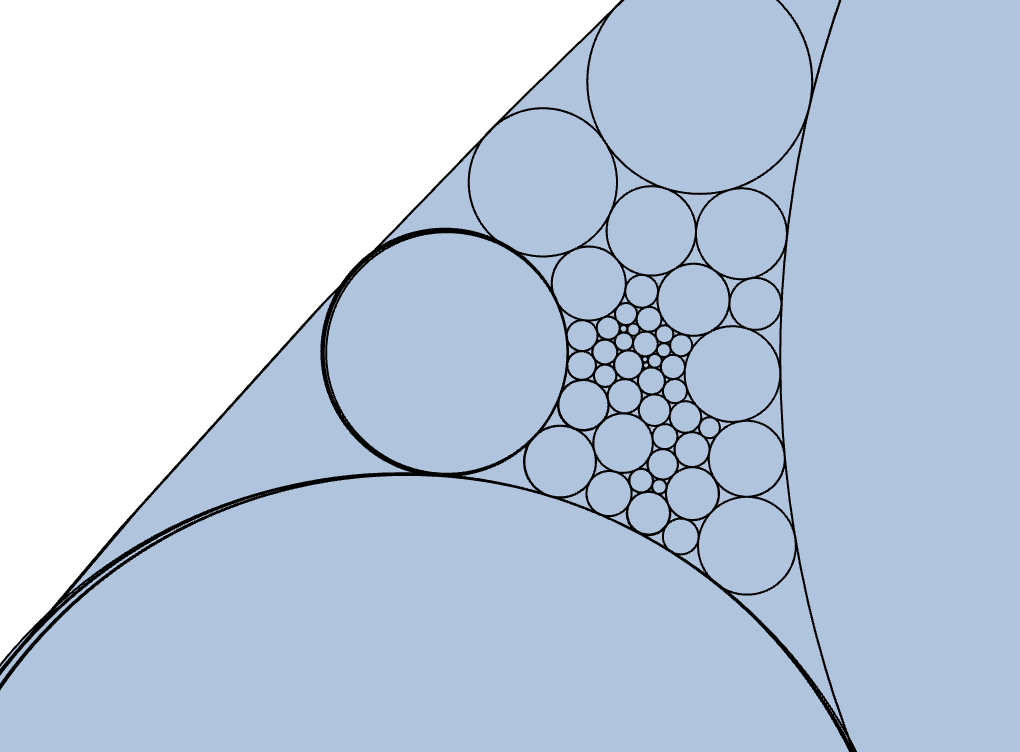
\includegraphics[width = 0.40\textwidth]{figures/mobius3.png}
        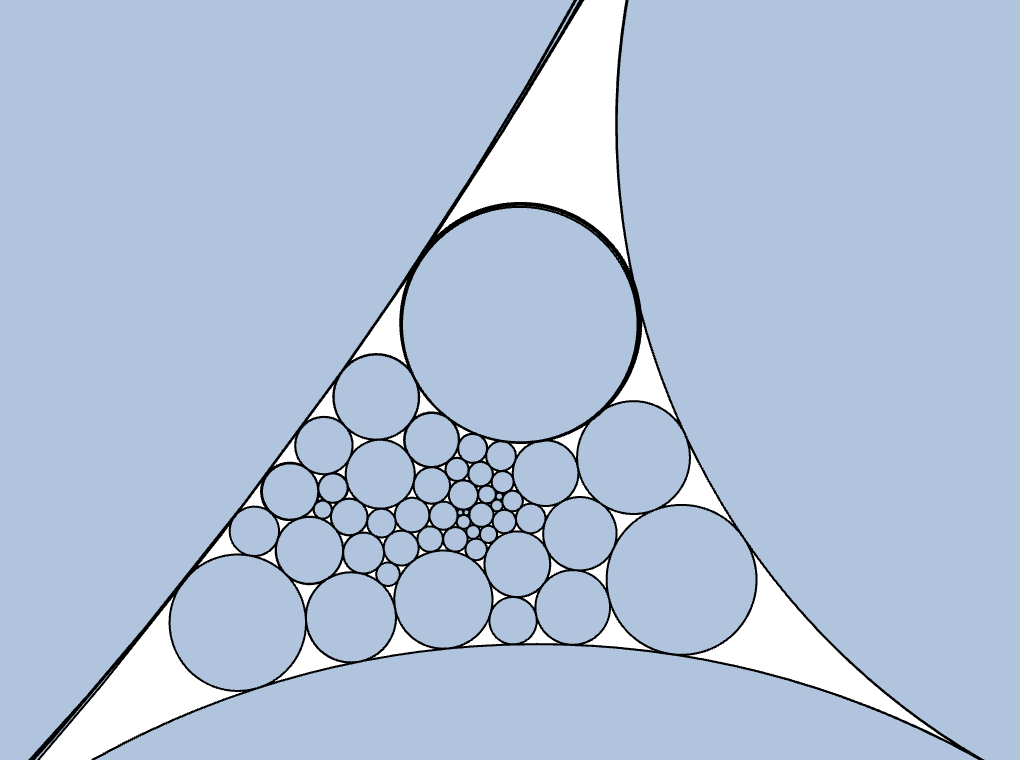
\includegraphics[width = 0.40\textwidth]{figures/mobius4.png}
      \caption{Two M\"{o}bius transformations of a circle packing.}
      \label{fig:mobius}
    \end{figure}

  \textbf{Dual Packings.} 
  \label{sub:dual_packings}
    Circle packings of triangulations always admit a \emph{dual packing} (Fig~\ref{fig:primal_dual}).
    By pressing the \texttt{'d'} key, the user can see the dual packing.
    \begin{figure}[ht]
      \centering
        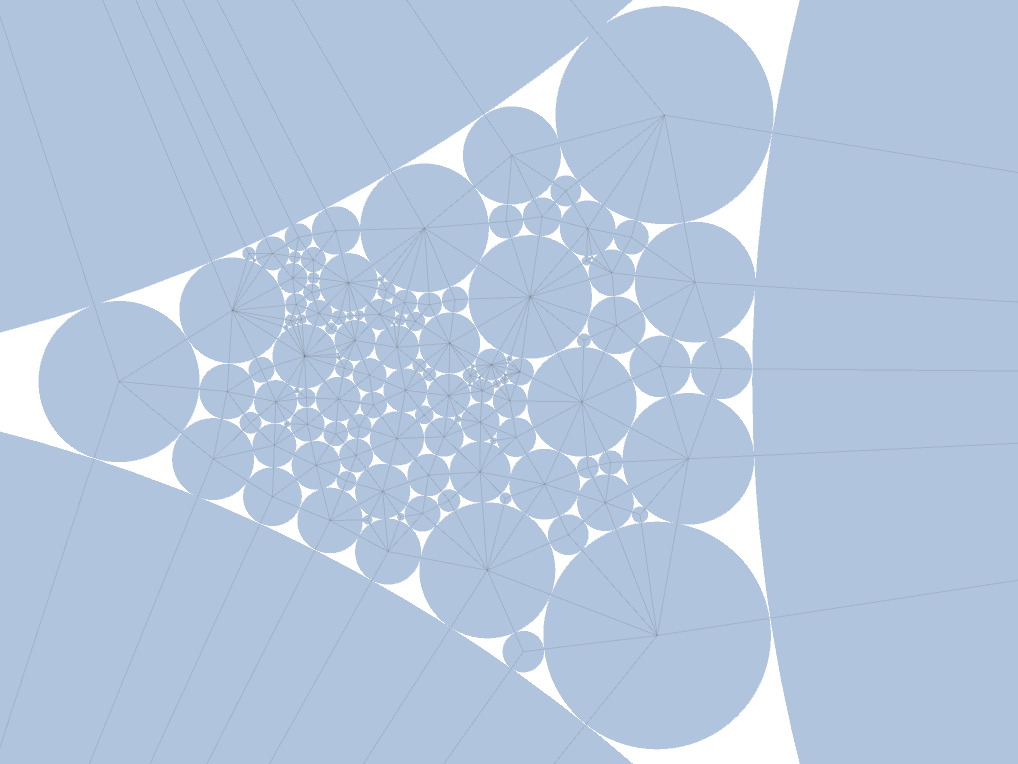
\includegraphics[width = 0.40\textwidth]{figures/primal.png}
        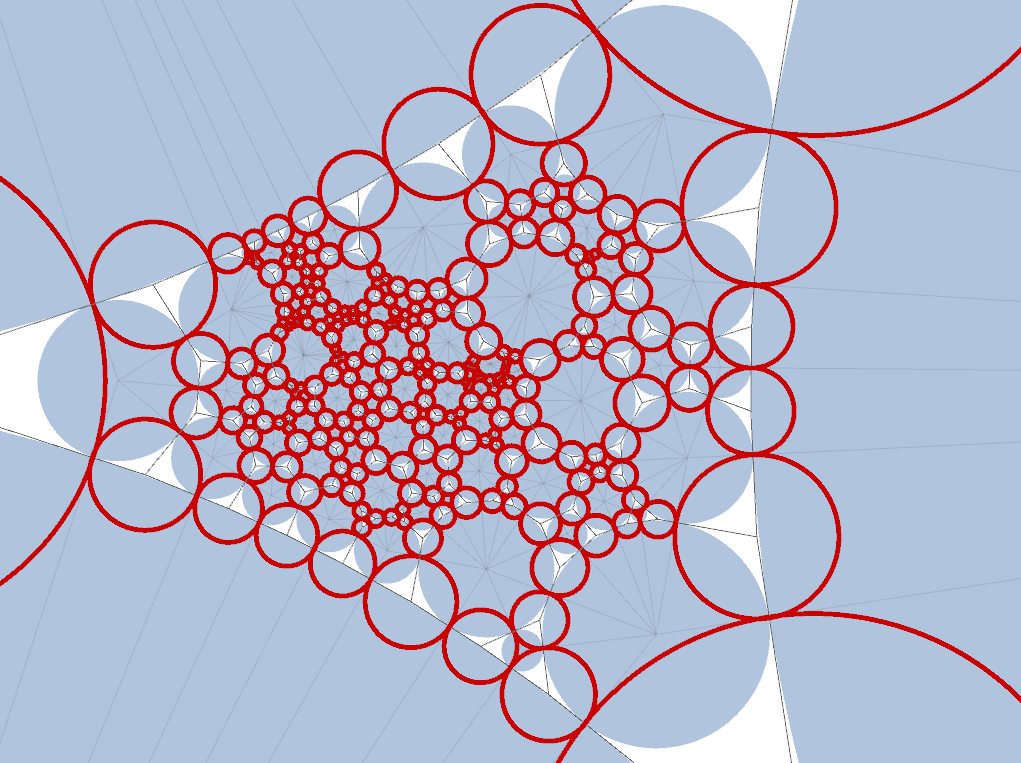
\includegraphics[width = 0.40\textwidth]{figures/dual.png}
      \caption{A packing and it's dual.}
      \label{fig:primal_dual}
    \end{figure}


\section{Interactive Input}
\label{sec:interactive_input}

  One immediate challenge to working interactively with circle packings is the need for input triangulations.
  We would like to be able to produce triangulations with a minimum of effort.  
  The most natural approach is to draw circles and produce the weighted Delaunay triangulation of the circles.
  Input is given by clicking a center and dragging to set the radius of an input disk.
  As new points are added, we incrementally compute the weighted Delaunay triangulation.
  An advantage of this approach is that it is very easy to draw approximate circle packings.  
  This allows one to experiment with examples where one has a clear idea of the expected output.

  \begin{figure}[ht]
    \centering
      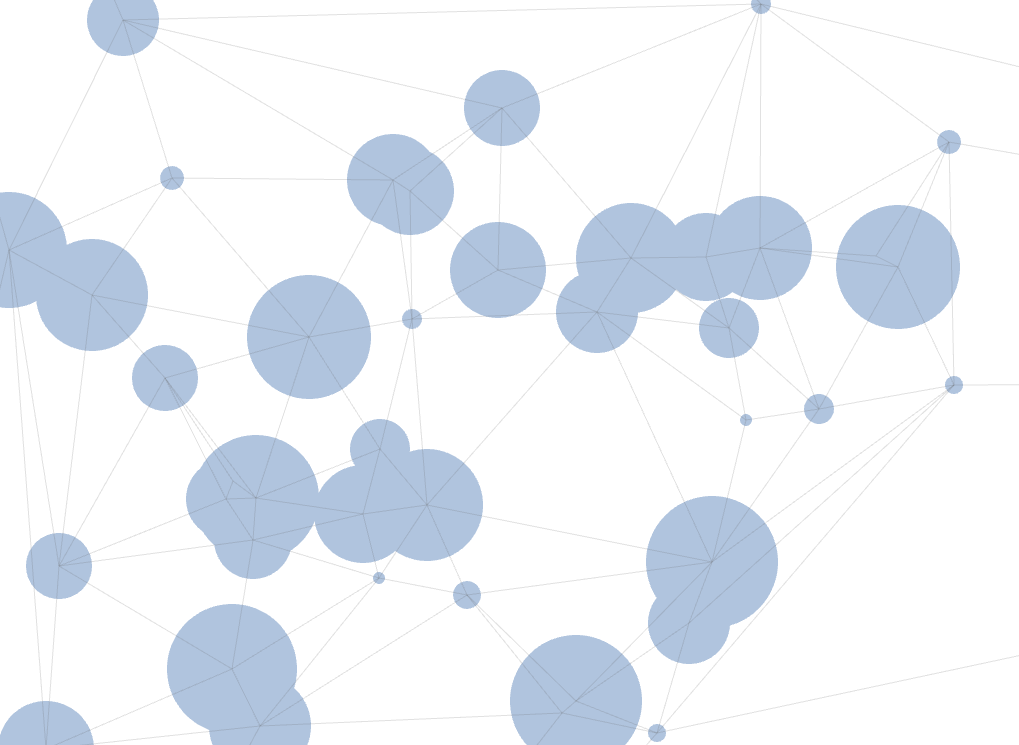
\includegraphics[width = 0.40\textwidth]{figures/input.png}
      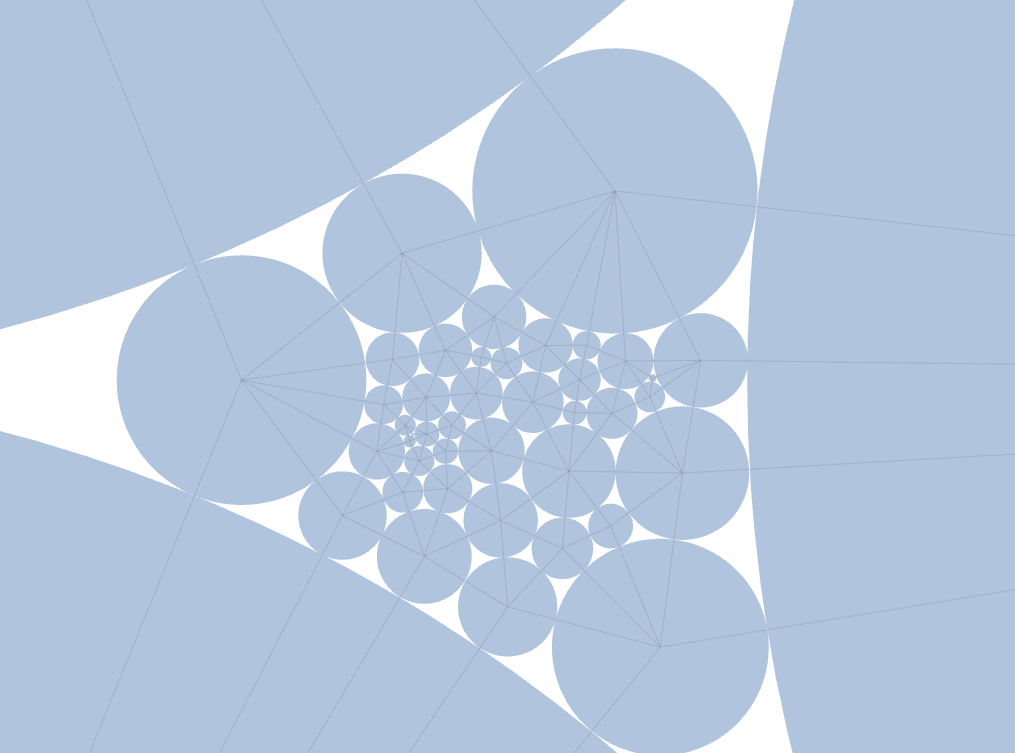
\includegraphics[width = 0.40\textwidth]{figures/output.png}
    \caption{An input of circles (left) and the circle packing output (right).}
    \label{fig:input_output}
  \end{figure}
  
  As a M\"{o}bius transformations will give new circle packings of the input graph, we allow the user to transform the plane to explore different packings.
  These transformations can be viewed by hitting the \texttt{'spacebar'} key twice to change views and then moving the mouse.
  
  If the user presses the \texttt{'spacebar'} key again, then dragging with the mouse will instead rotate a 3D view of the circle packing mapped stereographically onto a sphere.
  
\section{Algorithms}
\label{sec:algorithms}

  Currently we have two different algorithms implemented.
  The first is based on the algorithm from Stephenson~\cite{stephenson05introduction}.
  Given any set $\{r_1,\ldots, r_n\}$ of radii, it is possible to compute the angles of the triangles using the law of cosines.
  The final radii are those for which the angles at any vertex sum to exactly $2\pi$.
  Thus, the algorithm searches for the radii of the disks by making small incremental updates to the radii, increasing the radius if the angle sum is more than $2\pi$ and decreasing the radius of the angle sum is less than $2\pi$.
  
  The second algorithm is based on spring embeddings of graphs such Tutte's algorithm.
  In this algorithm, the embedded graph is interpreted as a system of springs. 
  This ``force-directed'' algorithm is not known to terminate, but it seems to be quite effective on small examples.


\section{Future Work} 
\label{sec:future_work}

  We are actively developing new features to provide both new ways to visualize the packings as well as new heuristics.
  The current implementation supports two of the major paradigms in circle packing algorithms.
  Next, we will consider algorithms based on discrete Ricci flow.
  
\bibliography{references}

\end{document}
